\documentclass{ctexart}

% 导入导言区设置
\usepackage{textcomp}    % 提供额外的文本符号
\usepackage{pdfpages}    % 允许将PDF文件作为页面导入到LaTeX文档中
\usepackage{fancyhdr}    % 提供自定义页眉页脚的功能
\usepackage{geometry}    % 用于设置页面尺寸、边距等页面布局参数
\usepackage{titlesec}    % 允许自定义章节标题的格式和样式
\usepackage{fontspec}    % XeLaTeX/LuaLaTeX下的字体设置包,支持系统字体和OpenType特性
\usepackage{xeCJK}       % 用于支持CJK文本的字体设置
\usepackage{amsmath}     % 支持 LaTeX 数学环境
\usepackage{tabularx}
\usepackage{multirow}
\usepackage{caption}
\usepackage{float}

% 设置目录深度,只显示到二级标题
\setcounter{tocdepth}{2}

% 定义字体
\setCJKmainfont{Songti SC}  % 调用宋体
\setmainfont{Times New Roman} % 西文主字体

% 定义纸张大小
% 论文采用A4纸打印。页边距:上3厘米,下2厘米,左3厘米,右2厘米;装订线1厘米;页眉距边界2厘米,页脚距边界1厘米。
\geometry{
  a4paper,            % A4纸张标准
  left=3cm,           % 左边距(含装订线)
  right=2cm,          % 右边距
  top=3cm,            % 上边距(页眉距纸张顶部2cm)
  bottom=2cm,         % 下边距(页脚距纸张底部1cm)
  bindingoffset=1cm,  % 装订线(在左边距基础上额外增加)
  headheight=0.8cm,   % 页眉内容区高度
  headsep=0.6cm,      % 页眉与正文间距(2cm页眉边界要求 - 0.8cm页眉高度 - 3cm上边距)
  footskip=1cm        % 页脚底部到页面底部的距离
}

% 设置摘要、目录等标题样式
% "摘要"、"目录"、 "致谢"、"参考文献","附录"等为黑体三号字,"ABSTRACT"为Times New Roman加黑三号字,均居中,单倍行距,段前2行,段后2行。
\renewcommand{\abstractname}{\heiti\zihao{3}\centering 摘要}
\newcommand{\engabstractname}{\selectfont\bfseries\zihao{3}\centering ABSTRACT}
\renewcommand{\contentsname}{\heiti\zihao{3}\centering 目录}
\newcommand{\acknowledgement}{\heiti\zihao{3}\centering 致谢}
\renewcommand{\appendixname}{\heiti\zihao{3}\centering 附录}
\renewcommand{\refname}{\heiti\zihao{3}\centering 参考文献} % 添加参考文献标题样式

% 配置页眉页脚样式
% 全文除封面、封底无页眉外,均采用页眉“杭州电子科技大学本科毕业论文”或“杭州电子科技大学本科毕业设计”。宋体五号字,居中。
% 封面、封底、中文摘要、ABSTRACT、目录无需页码,论文其余部分均采用阿拉伯数字页码,Times New Roman五号字,居中。
\pagestyle{fancy} % 设置页面样式为fancy(适用于除封面外的所有页面)
\fancyhf{}         % 清空默认页眉页脚设置
\fancyhead[C]{\songti\zihao{5}杭州电子科技大学本科毕业设计(论文)} % 页眉内容:宋体五号字,居中。
\renewcommand{\headrulewidth}{0.5pt} % 页眉装饰线粗细设置为0.5磅
% 重定义plain样式
\fancypagestyle{plain}{
  \fancyfoot[C]{\selectfont\zihao{5}\thepage} % Times New Roman五号字,居中。
  \renewcommand{\headrulewidth}{0.5pt} % 保留页眉装饰线
}

% 配置正文内容样式
% 正文内容中文为宋体小四号字,英文为Times New Roman小四号字,行距20磅,标准字符间距。每一章内容均另起一页。
\renewcommand{\normalsize}{\songti\zihao{-4}} % 设置正文默认字体为宋体小四号
\linespread{1.5} % 设置行距为20磅(约为1.5倍行距)
\let\originalsection\section
\renewcommand{\section}{\clearpage\originalsection} % 设置每章另起一页
\setlength{\parindent}{2em} % 设置首行缩进为2个汉字

% 配置正文标题样式
% 正文第一级标题为黑体三号字,居中,单倍行距,段前2行,段后2行。第二级标题为黑体四号字,第三级标题为黑体小四号字
\titleformat{\section}{\heiti\zihao{3}\centering}{\thesection}{1em}{} % 第一级标题为黑体三号字,居中,单倍行距
\titleformat{\subsection}{\heiti\zihao{4}}{\thesubsection}{1em}{} % 第二级标题为黑体四号字
\titleformat{\subsubsection}{\heiti\zihao{-4}}{\thesubsubsection}{1em}{} % 第三级标题为黑体小四号字



\begin{document}

% 封面页、陈诺书(无页码)

\includepdf[pages={1}]{./source/封面页.pdf}

\includepdf[pages={2}]{./source/封面页.pdf}
\setcounter{page}{0}   % 重置页码计数器

% 中文摘要
% 中文摘要内容为宋体小四号字,摘要内容后下空一行打印“关键词”为黑体小四号字,其后关键词为宋体小四号字;
\begin{abstract}
    \linespread{1.5}\selectfont % 设置行距为20磅
    {\songti\zihao{-4} % 设置宋体小四号字
    % 摘要内容
    本研究针对零售行业排班管理需求,探索构建了一套智能化排班解决方案。系统设计遵循业务导向原则,通过分层架构与模块化设计,尝试在多维度约束条件下寻求排班效率与合规性的平衡。

    在技术实现层面,系统采用前后端分离的设计思路:前端通过组件化界面实现排班过程的可视化交互,支持多维度数据展示与操作反馈;后端基于微服务架构构建弹性化业务中台,将员工管理、规则配置等核心功能模块解耦,通过领域驱动设计建立具有行业特征的数据模型。技术方案特别关注规则引擎与算法模块的协同机制,在确保劳动法规硬性约束的基础上,尝试通过智能算法实现人力需求与员工特征的动态适配。

    实际应用表明,该系统在规则碎片化管理、多门店协同等方面展现出一定应用价值。通过构建标准化的排班流程与灵活配置机制,既保留了传统排班工作模式的操作惯性,又为算法优化留有可拓展空间。特别是在应对节假日促销、员工突发请假等弹性需求场景时,系统提供的冲突预警与快速调整功能,有助于提升排班工作的容错性与可维护性。这些探索性实践为零售行业人力资源管理数字化转型提供了有益参考,其设计思路对服务业排班场景的技术改造具有一定借鉴意义。

    \vspace{\baselineskip} % 添加一个空行
    {\heiti\zihao{-4}关键词:} % 关键词标题:黑体小四号字
    {\songti\zihao{-4}智能排班系统;模拟退火算法;前后端分离;微服务架构} % 关键词内容:宋体小四号字,用分号分隔
    }
\end{abstract}
\clearpage

% 英文摘要
% 英文摘要内容为Times New Roman小四号字,英文摘要内容后下空一行打印“Keywords”为Times New Roman加黑小四号字,其后关键词为小写Times New Roman小四号字。
\renewcommand{\abstractname}{\engabstractname}  % 切换摘要标题为英文
\begin{abstract}
    \linespread{1.5}\selectfont % 设置行距为20磅
    {\selectfont\zihao{-4} % 设置 Times New Roman 小四号字
    % Abstract content
    This study explores the construction of an intelligent scheduling solution in response to the scheduling management needs of the retail industry. The system design follows the business-oriented principle, attempting to balance scheduling efficiency and compliance under multi-dimensional constraints through hierarchical architecture and modular design.

    On the technical implementation level, the system adopts a front-end and back-end separation design approach: the front end achieves visual interaction in the scheduling process through component-based interfaces, supporting multi-dimensional data display and operational feedback; the back end constructs an elastic business platform based on microservice architecture, decouples core functional modules such as employee management and rule configuration, and establishes data models with industry characteristics through domain-driven design. The technical solution pays special attention to the collaborative mechanism between the rule engine and the algorithm module, attempting to dynamically adapt labor demand and employee characteristics through intelligent algorithms while ensuring the rigid constraints of labor laws.

    Practical applications show that the system demonstrates certain application value in aspects such as rule fragment management and multi-store collaboration. By building standardized scheduling processes and flexible configuration mechanisms, it retains the operational inertia of traditional scheduling work modes while leaving room for algorithm optimization. Especially in response to flexible demand scenarios such as holiday promotions and sudden leave requests from employees, the system's conflict warning and rapid adjustment functions help improve the fault tolerance and maintainability of scheduling work. These exploratory practices provide a useful reference for the digital transformation of human resource management in the retail industry and have certain reference significance for the technical transformation of scheduling scenarios in the service industry.
    
    \vspace{\baselineskip} % 添加一个空行
    {\selectfont\bfseries\zihao{-4}Keywords:} % Keywords 标题:Times New Roman 加黑小四号字
    {\selectfont\zihao{-4}intelligent scheduling system; simulated annealing algorithm; front-end and back-end separation; microservices architecture} % 关键词内容:小写 Times New Roman 小四号字,用分号分隔
    }
\end{abstract}
\clearpage

% 摘要、目录(无页码)
\pagenumbering{gobble} % 禁用页码
\tableofcontents
\clearpage

% 正文开始
\pagenumbering{arabic}
\setcounter{page}{1} % 正文页码从1开始
\pagestyle{plain} % 使用重定义的plain样式

\section{绪论}
\subsection{研究背景}
随着社会经济的快速发展和各行业规模的不断扩大,人员排班问题已成为企业运营管理中的关键环节。在铁路运输领域,机车乘务员的排班直接关系到行车安全和运营效率\cite{1016279053.nh}。传统的人工排班方式不仅耗时耗力,且难以满足现代铁路运输的高效性和公平性需求。特别是在铁路运输规模不断扩大的背景下,手工排班已无法适应复杂的乘务规则和动态变化的工作量\cite{1016279053.nh}。因此,开发智能排班系统成为铁路信息化发展的必然趋势。
类似的问题也出现在航空和地铁运营领域。机场AOC(机场运行控制中心)在航班量激增的情况下,面临人员配置和排班的巨大挑战\cite{1022506340.nh}。传统的手工排班方式效率低下,且难以应对航班量的动态变化。地铁乘务员的排班同样复杂,需要考虑交路计划、工时均衡和休息时间等多重约束\cite{1014151664.nh}。这些行业的共同特点是排班问题具有多目标、多约束的特性,属于NP难问题,传统方法难以高效求解。
在医疗领域,护士排班问题同样备受关注。传统的人工排班模式无法满足护士的个性化需求,且容易导致疲劳和满意度下降\cite{GWYG202110011}。智能排班系统的引入可以有效优化人力资源配置,提高护士和患者的满意度。此外,银行业也面临着弹性排班的需求,如何在业务高峰期和低谷期合理配置人员成为管理难点\cite{1016015859.nh}。

\subsection{研究意义}
智能排班系统的研究和开发具有重要的理论意义和实际应用价值。从理论角度来看,排班问题属于多目标优化问题,涉及组合优化、运筹学等多个学科领域\cite{DNZS202202029}。通过研究智能排班算法,可以推动相关理论的发展,为解决其他复杂优化问题提供借鉴。例如,遗传算法、粒子群算法和模拟退火算法等在排班问题中的应用,不仅拓展了算法的适用范围,也为算法的改进和创新提供了实践基础\cite{RJDK202301028}。

从实际应用角度来看,智能排班系统可以显著提高排班效率和质量。在铁路运输领域,智能排班系统能够自动生成乘务计划,减少人工干预,确保乘务员的工作与休息时间均衡,防止疲劳驾驶,保障行车安全\cite{1016279053.nh}。在地铁运营中,智能排班系统可以优化交路计划和人员配置,提高运营效率和乘务员满意度\cite{1014151664.nh}。在医疗领域,智能排班系统可以根据护士的个性化需求生成排班方案,降低疲劳感,提高工作满意度\cite{GWYG202110011}。

此外,智能排班系统的应用还能带来显著的经济效益。例如,在银行业中,弹性排班系统可以根据业务量的动态变化调整人员配置,减少人力资源浪费,提高服务效率\cite{1016015859.nh}。在航空领域,智能排班系统可以优化AOC人员的配置,降低运营成本,提高航班保障能力\cite{1022506340.nh}。这些实际效益进一步凸显了智能排班系统研究和开发的重要性。

综上所述,智能排班系统的研究和开发不仅具有重要的理论意义,还能为各行业的运营管理提供高效、公平和灵活的解决方案,推动相关行业的信息化发展和效率提升。未来,随着人工智能和大数据技术的不断发展,智能排班系统将在更多领域发挥重要作用。



\subsection{国内外研究现状综述}
\subsubsection{国内研究现状}
在铁路运输领域,王兴慧(2016)开发的机车乘务员智能排班系统通过计算机自动生成排班计划,有效解决了传统手工排班效率低下、难以优化的问题\cite{1016279053.nh}。该系统综合考虑乘务员作息时间均衡性,防止疲劳驾驶,已在铁路系统得到应用。研究指出,该系统使排班时间从原来的数小时缩短至分钟级,乘务员工作时间均衡度提升35\%。

民航领域的排班研究相对较新。熊静(2022)针对机场AOC人员排班问题,创新性地将改进遗传算法应用于多目标优化模型\cite{1022506340.nh}。通过动态调整交叉和变异算子,算法收敛速度提升40\%,在保证排班经济性的同时,使员工时长方差减少24\%,早晚班安排合理性显著提高。

地铁系统的排班研究更具实践性。潘云龙(2013)设计的沈阳地铁智能排班系统采用遗传算法自动生成乘务交路,将传统需要2-3天的人工排班工作压缩至1小时内完成\cite{1014151664.nh}。系统还集成出退勤管理、公里统计等辅助功能,实际应用显示排班准确率达到98.7\%。

在医疗服务领域,王莹等(2021)开发的超声科智能排班系统实现了人力资源的数字化管理\cite{XHYX202106028}。通过整合医师资质、设备状态等多维数据,系统使排班满意度从68\%提升至92\%,同时减少管理人员30\%的工作量。

商业银行的排班研究则侧重弹性管理。林畅(2015)基于B/S架构开发的银行排班系统,采用贪婪算法动态调整窗口服务人员\cite{1016015859.nh}。在某商业银行试点中,客户平均等待时间缩短40\%,同时人力成本降低15\%。

\subsubsection{国外研究现状}
国外学者在智能排班系统的理论研究方面取得显著进展,主要研究方向集中在以下领域:

Gao等人在能源效率调度领域的研究表明,群体智能算法在复杂调度问题中展现出显著优势\cite{Gao2020}。其研究指出,通过智能机器开关策略可降低非生产时段能耗达23\%,这对零售业排班系统的绿色计算具有重要启示。

Cunha等人提出的强化学习方法\cite{app11083710}创新性地将马尔可夫决策过程与排班问题结合,在作业车间调度场景中实现秒级响应。实验数据显示该方法解的质量接近传统模拟退火算法,为动态排班需求提供了新思路。

Fu等人系统分析了多工厂协同调度问题\cite{9409755},发现遗传算法在解决运输约束和异构工厂协同问题上表现突出。其研究指出分布式调度可使资源利用率提升18\%,这对连锁零售企业的多门店排班具有借鉴意义。

现有方法在动态环境适应性方面仍存在局限,未来可结合模拟退火算法的全局搜索能力与强化学习的实时响应特性,构建混合优化模型。这种技术融合将为智能排班系统提供更强大的动态调度能力。

\subsection{研究的主要目标}

本研究立足于零售行业实际运营需求,针对传统排班方式存在的效率瓶颈与管理痛点,致力于探索一套切实可行的智能化排班解决方案。研究过程始终以解决企业现实问题为根本导向,力求在现有技术条件与业务场景之间找到平衡点,而非片面追求算法复杂度或理论创新。具体而言,本研究主要围绕以下三个层面展开目标设定:

在业务应用层面,研究旨在构建符合零售行业特性的排班管理机制。针对零售门店多班次运转、员工技能差异、临时调班频繁等特点,着力设计具有实用价值的排班规则体系。重点解决排班过程中普遍存在的岗位匹配度低、工时分配不均、突发调整困难等实际问题,力求在合规性要求与运营灵活性之间寻求平衡。通过建立标准化的排班流程,帮助企业减少人为操作失误,降低排班管理的时间成本。

在技术实现层面,研究着重探索适应中小型零售企业技术基础的解决方案。考虑到多数零售企业信息化水平参差不齐的现状,系统设计强调技术方案的适用性与可操作性。采用渐进式改进策略,在保留传统排班工作模式核心要素的基础上,逐步引入智能化辅助功能。通过可视化排班界面、自动化冲突检测等功能的实现,帮助管理人员从繁琐的重复劳动中解脱,将工作重心转向决策优化。同时注重系统的易维护性,确保非技术人员也能完成日常运维操作。

在算法优化层面,研究重点关注排班模型的实际应用效果。相较于追求算法理论层面的突破,更注重算法在实际场景中的适应能力。针对零售排班中普遍存在的动态调整需求,着力提升算法对临时变更的响应速度与处理能力。通过构建合理的约束条件体系,确保算法生成的排班方案既满足企业用工需求,又能兼顾员工合理诉求。在保证排班质量的前提下,将计算耗时控制在管理人员可接受范围内,避免因过度优化影响系统实用性。

研究特别关注系统在不同规模零售场景中的适应性。对于小型社区门店,系统侧重快速排班与灵活调整功能的实现;针对连锁品牌门店,则强化多店协同排班与人力共享机制。通过模块化设计,使系统既能满足单店独立运营需求,也可支持区域化集中管理。在算法参数设置上预留调整空间,允许企业根据自身特点设置不同的优先级权重,如将员工偏好、工时均衡或人力成本等要素进行差异化配置。

整体而言,本研究不追求构建理论意义上的"最优"排班系统,而是致力于开发具有实用价值的"适用"解决方案。通过将先进算法与行业经验相结合,在技术可行性与管理有效性之间寻找最大公约数,最终形成企业用得上、员工愿意用、管理者能操作的智能化排班工具。这种立足现实需求、强调渐进改良的研究路径,或许能为零售行业的数字化转型提供更具实践价值的参考。

\subsection{论文的主要内容与结构安排}
本文围绕零售行业智能排班系统的设计与实现展开研究,采用循序渐进的方式逐步深入探讨系统建设的各个环节。全文共分为八个主要章节。

第一章为绪论部分,主要阐述研究的背景动因和整体构想。从零售行业排班管理的实际痛点出发,分析传统排班方式面临的效率瓶颈,说明开展智能排班系统研究的必要性。同时介绍研究的理论意义和实践价值,梳理国内外相关领域的研究进展,为后续研究奠定基础。

第二章重点说明研究目标和整体规划。明确系统建设的主要方向和使用场景,着眼于解决企业日常排班中的具体困难,力求在现有技术条件下找到最合适的解决方案。

第三章介绍系统开发涉及的关键技术。采用通俗易懂的语言解释模拟退火算法、前后端分离架构等核心技术原理,着重说明这些技术如何与排班场景相结合。避免深奥的理论推导,更多从实际应用角度分析技术选型的合理性。

第四章开展系统需求分析工作。通过与零售企业管理者和一线员工的深入交流,梳理排班业务的核心流程和关键需求。从用户角度出发,详细描述系统应具备的各项功能,分析系统建设的可行性和实施路径。

第五章重点研究模拟退火算法在排班系统中的应用。针对零售排班的特点,设计适合的算法模型,探讨如何将排班规则转化为算法可处理的约束条件。通过实际案例验证算法的有效性和适用性。

第六章详细阐述系统的设计与实现过程。介绍系统的整体架构设计思路,说明各功能模块的实现方法。包括前端界面的交互设计、后端服务的功能划分、数据库的结构设计等具体内容,展现系统从设计到落地的完整过程。

第七章展示系统实际运行效果。通过界面截图和功能演示,直观呈现系统的工作流程和使用方法。重点说明系统如何帮助用户完成日常排班工作,解决实际问题。

第八章总结全文研究成果,客观评价系统的优点与不足。提出未来改进方向和应用展望,为后续研究提供参考建议。

附录部分包含系统设计的补充材料,如详细功能说明、核心算法描述等,为有兴趣深入了解的读者提供更多参考信息。

\section{相关技术与理论基础}
\subsection{模拟退火算法}
\subsubsection{算法简介}
模拟退火算法是一种受自然界物理现象启发的优化方法。其灵感来源于金属冶炼中的退火工艺——先将金属加热至高温使其原子处于活跃状态,再缓慢降温使原子逐渐趋于稳定排列,最终获得结构完整的晶体。科学家们观察到,这种物理过程中的能量状态变化与数学优化问题存在相似性,于是将其原理抽象为一种寻找全局最优解的算法。

在计算机科学领域,模拟退火主要应用于解决复杂的组合优化问题。这类问题往往存在大量可能的解,且解与解之间通过特定规则相互关联,如同排班系统中每个班次安排都会影响整体排班方案的合理性。与传统穷举法相比,模拟退火通过引入"温度"参数控制搜索过程,既允许向更优解的方向探索,也以一定概率接受暂时性的劣化解,这种特性使其能够有效跳出局部最优陷阱。

对于排班系统这类包含多维度约束的优化场景,模拟退火算法展现出独特的适用性。例如在零售门店排班中,既要满足不同时段的岗位人力需求,又要兼顾员工的工作偏好,还要考虑劳动法规对工作时长的限制。算法通过模拟金属冷却的渐进过程,逐步调整排班方案的各个要素,如同经验丰富的排班员在不断试错中寻找平衡点。这种渐进式优化的特性,使得算法既能保持全局搜索能力,又能避免完全随机搜索的低效性。

\subsubsection{算法机制}
模拟退火算法的运行机制可以形象地比喻为一个精益求精的工匠打磨作品的过程。在排班系统的应用中,算法首先会生成一个初始排班方案,这个方案可能就像新手排班员初次制定的草稿——虽然满足基本要求,但存在诸多可以改进之处。此时的"温度"参数较高,相当于工匠刚开始加热材料,允许进行大刀阔斧的调整。

随着算法迭代,系统会逐步生成新的候选方案。例如随机调换两名员工的班次,或调整某个时段的岗位配置。每次调整后,算法会像质检员一样评估新方案的优劣:如果调整后更符合预期目标(如工时更均衡、人力成本更低),就欣然采纳;即使调整后效果暂时变差,也会根据当前"温度"计算出一个接受概率——温度高时接受概率大,如同工匠在材料较软时允许较大变形,温度降低后则趋于保守。

这种机制在排班系统中体现为对创新方案的包容性。例如某个临时调整可能导致当日人力成本上升,但可能为后续班次优化创造机会。算法通过概率性的接受策略,既保持了对解空间的探索热情,又避免了在局部最优解上过早固步自封。就像老练的排班主管,既懂得坚持基本原则,又能在必要时灵活变通。

降温策略是算法控制优化节奏的关键。常见的做法是逐步降低温度参数,如同工匠掌握火候般调节加热强度。在排班应用中,这相当于优化过程从初期的广泛尝试转向后期的精细调整。当温度降至设定阈值时,算法如同完成冷却的金属,呈现出相对稳定的优化结果。整个过程需要精心设计温度下降曲线,既保证足够时间探索可能解,又避免无谓的重复计算。

\subsubsection{算法优缺点}
模拟退火算法在排班系统中的应用具有显著优势。首要特点是其跳出局部最优的能力,这就像经验丰富的排班专家不会被既有思维局限,总能找到突破常规的新思路。对于存在多个约束条件的排班问题,算法能够通过概率性接受机制,穿越目标函数的"山谷丘陵",最终抵达更优解区域。这种特性在处理员工突发请假、临时调班等动态需求时尤为重要。

另一个优势是算法的灵活性。不同于某些需要严格数学模型的优化方法,模拟退火对目标函数的形式要求较低。在排班系统中,管理者可以自由定义各种评价指标的组合,如将员工满意度、人力成本、法规遵从度等要素按需加权。这就像为排班员提供了一套可定制的评价标准,既考虑企业运营需求,也兼顾员工个人诉求。

但算法也存在需要正视的局限性。计算效率问题首当其冲,尤其在处理大规模排班场景时,可能需要较长的优化时间。这如同让一位精益求精的工匠精雕细琢每处细节,虽然成品质量上乘,但耗时较久。对于需要快速响应的实时排班需求,可能需要结合其他优化策略进行补充。

参数调优的敏感性是另一个挑战。温度初值、降温速率等参数的设置直接影响优化效果,这需要开发者对业务场景有深刻理解。就像新手厨师掌握火候需要反复练习,算法参数的调整也需要结合具体排班需求不断试验。此外,算法本质上属于启发式方法,不能保证绝对最优解的获取,这在追求极致优化的场景中可能成为制约因素。

在零售排班系统的具体实践中,这些特性需要辩证看待。模拟退火算法的全局搜索能力,使其特别适合处理多门店协同、动态调班等复杂场景。而计算效率方面的局限,则可以通过合理设置迭代次数、采用分布式计算等工程手段进行缓解。正如老练的排班主管懂得权衡时间成本与方案质量,算法应用也需要在优化精度与计算效率之间寻找平衡点。

\subsection{基于Vue.js的前端工程化实现}

\subsubsection{框架概述}

Vue.js作为渐进式前端框架,为复杂应用的构建提供了温和的技术路径。其核心设计理念强调"渐进式"的框架演进思路,允许开发者根据项目需求灵活选择功能模块,这种可插拔的特性使其特别适合中小型项目的技术选型。在智能排班系统的前端实践中,Vue.js展现出的视图层解决方案,为管理系统的可视化界面开发提供了可靠基础。

与传统前端开发模式相比,Vue.js通过声明式渲染和组件化开发模式,显著降低了视图与数据状态同步的复杂度。在排班系统的具体场景中,这种特性体现为排班表格的动态渲染效率提升——当后台排班数据发生变化时,系统能够自动完成界面元素的更新,而无需开发者手动操作DOM元素。这种数据驱动的开发范式,使得开发团队能够将更多精力聚焦于业务逻辑的实现,而非界面更新的技术细节。

组件化架构是Vue.js的另一重要特性,这一设计思想与排班系统的功能需求高度契合。例如,将排班日历、员工信息卡片、操作工具栏等界面元素封装为独立组件,既保证了功能的独立性,又实现了跨模块的复用。在开发实践中,这种模块化构建方式有效提升了代码的可维护性,特别是在处理多门店排班视图切换等复杂交互场景时,组件间的通信机制确保了功能扩展的灵活性。这种开发模式为后续功能迭代预留了充足空间,当需要新增排班规则配置模块时,可以通过组合现有组件快速实现功能扩展。

\subsubsection{架构设计和技术实现}

在工程实践中,采用分层架构设计是保证前端工程化质量的关键。系统前端架构主要划分为视图层、逻辑层和数据层三个层次,这种分层模式借鉴了传统MVC架构的设计思想,但根据Vue.js的特性进行了适应性改进。视图层专注于界面元素的呈现,通过模板语法声明式地描述UI结构;逻辑层处理业务规则和用户交互,采用选项式API组织组件行为;数据层则通过Pinia状态管理库实现跨组件状态共享,这种职责分离的设计原则确保了系统的可维护性。

组件通信机制的设计是架构实现的重点。在排班系统的复杂交互场景中,父子组件间的props传参与事件派发机制构成了基础通信渠道。例如,当用户在排班日历组件中选择特定日期时,通过自定义事件将日期参数传递给父组件,触发排班数据的重新加载。对于跨层级组件的状态共享需求,则引入Vuex进行集中式状态管理,将排班数据、用户权限等全局状态存储在单一数据源中。这种混合式通信方案在保证组件独立性的同时,有效解决了跨模块数据同步的难题。

工程化实践的另一个重要维度是构建流程的优化。通过Vite模块打包工具的深度整合,实现了开发环境的热重载和生产环境的代码优化。在开发阶段,利用Vite提供的脚手架工具快速搭建工程结构,其预设的Babel转译、ESLint校验等配置为代码质量提供了基础保障。针对排班系统特有的性能需求,特别对组件异步加载机制进行了优化,将非首屏组件进行代码分割,显著提升了页面初始加载速度。这种工程化实践使得系统在保持功能复杂度的同时,仍能提供流畅的用户体验。

\subsubsection{生态系统以及工具}

Vue.js生态系统的丰富性为工程实践提供了有力支撑。官方维护的Vue Router路由库在排班系统的多视图管理方面发挥了重要作用,其嵌套路由机制完美适配了系统复杂的导航结构。例如,将门店管理、员工档案等模块配置为独立路由节点,配合路由守卫实现权限控制,确保了不同角色用户访问路径的安全性。这种路由方案的实施,使得系统在功能扩展时能够保持导航结构的清晰度。

第三方组件库的选择与应用体现了技术选型的务实态度。在UI框架的选型过程中,经过对多种方案的实践比较,最终选用Element Plus作为基础组件库。其表单组件和表格组件的增强功能,极大提升了排班规则配置模块的开发效率。特别是可编辑表格组件,在排班方案的手动调整场景中表现出良好的交互体验。这种选择并非追求技术新颖性,而是基于组件稳定性与开发效率的平衡考量。

开发工具链的完善是提升工程效率的关键因素。Vue Devtools调试工具的深度使用,为组件层级审查和状态追踪提供了可视化支持。在排班日历组件的开发过程中,通过该工具的状态快照功能,快速定位了某次排班数据更新异常的问题根源。此外,配合VS Code编辑器的Vetur插件支持,实现了模板语法的高亮提示和代码片段自动补全,这些看似细微的工具改进,在实际开发中显著降低了编码错误率。


\subsection{基于Node.js的后端服务架构}
\subsubsection{框架概述}
Node.js作为轻量级后端运行环境,其设计理念体现出对现代软件开发需求的深刻理解。与传统后端技术相比,它采用独特的异步事件驱动架构,这种设计思路源自对高并发场景下资源利用效率的持续探索。在零售行业智能化转型过程中,这种运行环境展现出良好的适应性,尤其是在处理实时性要求较高的排班调整请求时,能够较好地平衡响应速度与资源消耗。

从技术演进的角度来看,Node.js的诞生并非要取代传统后端技术栈,而是为特定场景提供更优解决方案。其核心基于Google Chrome浏览器的V8引擎,这使得JavaScript语言突破了浏览器环境的限制,能够在服务端执行复杂逻辑。对于中小型系统而言,这种技术选型降低了全栈开发的门槛,开发者可以使用统一的语言进行前后端开发,这在智能排班系统的原型验证阶段体现出显著优势。当系统需要快速迭代时,这种技术统一性能够有效缩短开发周期。

在服务端应用场景中,Node.js表现出与传统多线程模型截然不同的处理方式。其单线程事件循环机制,类似于经验丰富的调度员在处理多任务时的思维方式——不执着于逐个完成任务,而是善于统筹安排。当面对排班系统常见的突发性调班请求时,这种机制能够避免因个别复杂操作阻塞整个系统,保持服务响应的连贯性。这种特性在处理人力资源管理系统常见的高并发读取操作(如批量查询员工可用时段)时尤为有利。

值得注意的是,Node.js生态系统的开放性为技术选型提供了充分灵活性。npm包管理仓库中丰富的第三方模块,如同专业工具库中琳琅满目的工具,开发者可以根据具体需求选择合适组件。例如在排班系统中,采用Express框架搭建基础服务结构,配合中间件机制实现请求过滤和权限验证,这种模块化组合方式既保证了核心功能的稳定性,又为后续功能扩展预留空间。这种渐进式的架构演进思路,与中小型项目"小步快跑"的开发节奏十分契合。

\subsubsection{核心特性}
事件驱动与非阻塞I/O模型构成了Node.js最为显著的技术特征,这种设计哲学在排班系统的后台服务中展现出独特价值。当系统需要同时处理多个排班调整请求时,传统同步处理方式容易造成请求堆积,而事件驱动机制如同经验丰富的交通指挥员,能够合理安排每个请求的处理顺序。例如在节假日促销期间,当多个门店同时发起紧急排班需求时,系统仍能保持平稳运行,避免出现服务响应延迟。

单线程事件循环机制虽然看似与传统并发模型背道而驰,实则蕴含着对系统资源利用效率的深刻考量。在排班系统的实际运行中,多数业务操作(如排班规则校验、员工信息查询)都属于I/O密集型任务,而非计算密集型任务。这种机制使得系统能够用较少资源支撑较高并发量,就像精明的商家善于用有限人手处理高峰客流。当处理员工批量导入这样的常规操作时,系统可以并行处理文件解析与数据库写入,显著提升整体处理效率。

模块化设计思想贯穿Node.js的各个层面,这种"分而治之"的哲学在复杂系统构建中尤为重要。在排班系统的服务端开发中,将员工管理、权限认证等功能模块进行物理隔离,通过清晰的接口定义实现模块间通信。这如同建造模块化建筑,每个功能单元保持独立又可灵活组合。当需要新增考勤统计功能时,只需在现有架构中添加对应模块,而无需重构整个系统。这种设计方式特别适合需求可能持续演进的智能化管理系统。

跨平台运行能力是Node.js的另一个基础特性,这种可移植性为系统部署提供了更多选择。在零售企业信息化水平参差不齐的现实情况下,系统可能需要部署在Windows服务器或Linux集群等不同环境。Node.js的跨平台特性如同万能适配器,确保服务在各种环境下保持稳定运行。这对于需要支持多门店异构IT环境的排班系统而言,显著降低了运维复杂度。当企业IT基础设施升级时,这种特性也保障了系统的平滑迁移能力。

\subsubsection{框架优点}
在资源利用效率方面,Node.js展现出轻量级技术的独特优势。相较于传统应用服务器,其运行时内存占用更为精简,这如同节能型设备在保证性能的同时降低能耗。对于中小型零售企业而言,这意味着可以用更经济的硬件配置承载智能排班系统,降低数字化转型的硬件投入门槛。当系统需要横向扩展时,这种轻量特性也便于实施容器化部署,提高资源利用率。

异步编程模型带来的高并发处理能力,在排班系统的典型应用场景中具有现实意义。当系统需要同时响应门店管理端的排班查询和员工移动端的班次确认时,非阻塞处理方式能够有效避免请求堵塞。这种特性如同超市收银台开设快速通道,让简单事务快速通过,复杂操作有序排队。特别是在业务高峰期(如月末排班计划制定时段),这种处理机制能够保障核心功能的可用性。

前后端技术栈的统一性带来的开发效率提升,在项目实践中的价值不容小觑。全栈开发者可以深入参与数据库设计、业务逻辑实现和接口规范制定等多个环节,这种技术连贯性减少了不同技术团队间的沟通损耗。在排班系统的开发过程中,从员工信息管理模块到排班算法服务的实现,采用统一技术栈有效保障了代码风格的一致性,降低了后期维护成本。当需要快速实现原型验证时,这种优势体现得尤为明显。

\subsection{微服务架构}
\subsubsection{架构概述}
微服务架构作为一种软件设计范式,其核心思想在于将复杂系统拆解为多个相对独立的服务单元。这种架构风格的形成,源自于软件开发领域对系统灵活性和可维护性的持续追求。在传统单体架构中,系统各个功能模块往往紧密耦合,任何局部修改都可能引发牵一发而动全身的连锁反应。微服务架构尝试通过业务边界的合理划分,为系统演进提供更从容的调整空间。

在零售行业智能排班系统的建设实践中,采用微服务架构的初衷并非追求技术潮流,而是基于实际需求的审慎选择。排班业务本身具有多维度特征:员工管理需要处理大量动态信息,排班规则需要适应不同门店的特殊要求,算法引擎则需要独立进行复杂计算。将这些功能模块集中部署,不仅会增加系统运行时的资源消耗,更会在功能迭代时形成相互制约。微服务架构的引入,为这些业务组件的独立发展提供了可能。

这种架构模式与排班系统的业务特性形成良好呼应。例如,员工信息管理作为基础服务,需要保持高可用性和数据一致性;排班规则引擎作为核心服务,需要具备快速响应和弹性扩展能力;而智能算法服务作为计算密集型模块,则需要与其他服务保持适度隔离。通过服务边界的合理划分,系统既保持了整体功能的完整性,又为各业务模块的独立优化创造了条件。

\subsubsection{设计原则}
在微服务架构的实施过程中,首要任务是建立清晰的服务划分标准。这需要开发团队深入理解业务本质,避免陷入技术层面的过度设计。对于排班系统而言,服务拆分主要遵循业务能力导向原则:将员工档案管理、门店配置管理、排班规则库等核心业务能力封装为独立服务。每个服务对应明确的业务职责,既保持功能的内聚性,又降低服务间的依赖性。

服务间的通信机制设计是架构落地的关键环节。在排班系统的具体实践中,主要采用两种交互模式:对于实时性要求较高的操作(如排班方案生成),采用同步通信机制保证响应速度;对于数据更新类操作(如员工信息变更),则采用异步消息队列实现最终一致性。这种混合式通信策略,既满足了核心业务流程的时效性要求,又缓解了系统在高并发场景下的压力。

在服务自治性方面,系统设计强调各微服务的独立进化能力。每个服务都配备专属的数据存储,例如员工服务独立维护人员信息数据库,排班服务则管理排班记录和规则配置。这种数据隔离策略虽然增加了部分数据同步的工作量,但有效避免了服务间的数据耦合。当某个服务需要调整数据模型时,只需确保接口契约的稳定性,而无需协调其他服务的改造。

\subsubsection{实现方式}
微服务架构的具体落地,需要平衡技术先进性与实施可行性之间的关系。在排班系统的技术选型中,主要采用轻量级容器化技术实现服务部署,这种方式既能保证环境一致性,又不会给运维团队带来过高学习成本。每个微服务封装为独立容器,通过标准化接口与其他服务交互,这种部署模式为系统的横向扩展提供了便利。

在服务治理方面,系统采用渐进式改进策略。初期重点建设服务注册与发现机制,确保服务之间的可寻址性;随着系统规模扩大,逐步引入熔断机制和流量控制功能。例如,在算法服务调用量激增时,系统能自动进行请求排队,避免服务雪崩效应。这种分阶段实施的治理策略,既控制了初期实施难度,又为后续优化预留了空间。

面对分布式系统固有的复杂性,团队采取了务实的应对措施。在事务管理方面,优先保证核心业务流程的最终一致性,通过补偿机制处理异常场景。例如生成排班方案时,若某个服务暂时不可用,系统会保留中间状态并自动重试,而非强求实时完成所有操作。这种设计选择虽然牺牲了部分实时性,但显著提高了系统的整体可用性。

\subsubsection{优势与挑战}
微服务架构为排班系统带来的核心价值,主要体现在系统演进能力的提升。当需要调整排班规则时,只需修改规则服务而无需重启整个系统;当算法模块需要升级时,可以独立部署新版本进行灰度测试。这种模块化演进能力,使得系统能够更好地适应零售行业快速变化的业务需求。特别是在应对节假日促销等特殊场景时,服务独立扩缩容的特性为系统稳定性提供了有力保障。

但架构优势的获得并非没有代价。服务拆分带来的运维复杂度提升,要求团队建立新的协作模式。开发人员需要从单体应用的思维惯性中转变,既要关注自身服务的功能实现,又要考虑服务间的协同配合。例如在接口版本管理上,团队制定了严格的兼容性规范,避免因接口变更引发级联故障。这些实践经验的积累,成为架构成功落地的重要支撑。

经过项目实践,我们认识到微服务架构并非银弹,其价值实现需要与具体业务场景深度契合。对于中小型排班系统,服务拆分应保持适度原则,避免过度设计带来的管理负担。在未来的系统演进中,将根据业务发展需要动态调整架构形态,在模块独立性与系统整体性之间寻求最佳平衡点。这种务实的技术路线选择,或许能为类似系统的架构设计提供有益参考。

\section{系统分析}
\subsection{系统设计原则}
系统的开发要遵守一定的标准,本系统的开发基于标准的软件工程项目开发规范,将整体的开发过程分为了需求分析、总体设计、系统功能实现、系统测试等相关流程。在具体的程序设计过程中,要遵循以下设计原则:
\begin{itemize}
    \item 第一,规范开发流程。严格遵循软件工程规范,建立需求分析、方案设计、编码实现到测试验证的全流程管理体系。通过定期需求评审与原型验证,确保各阶段产出物与用户预期高度契合,特别是在排班规则管理等核心模块的开发中,始终保持业务需求与技术实现的同步对齐。
    
    \item 第二,强化数据可靠性。采用事务机制与版本控制技术,构建从数据录入、存储到应用的全生命周期保障体系。在排班方案生成等关键操作中,通过数据库锁机制与操作日志追踪,有效防范并发场景下的数据不一致问题,为系统决策提供可信数据支撑。
    
    \item 第三,注重使用体验。针对零售行业用户的信息化水平特点,在界面设计和操作流程中贯彻"最小学习成本"理念。通过可视化排班视图、智能冲突提示等交互设计,降低非技术用户的操作门槛,使店长等基层管理人员经过简短培训即可熟练完成日常排班工作。
    
    \item 第四,优化性能指标。在满足功能完备性的基础上,重点提升系统响应速度与稳定性。采用异步计算、缓存策略等技术手段,将大规模排班方案的生成时间控制在分钟级,确保系统在高并发访问场景下仍能保持流畅操作体验。
\end{itemize}

\subsection{系统设计方案}
本系统的设计方案主要参考了软件工程的标准开发流程,结合零售行业排班管理的实际需求,采用分阶段实施的方式推进。具体开发过程分为四个主要环节:

\begin{itemize}
    \item 系统分析阶段:重点考察技术方案的可行性,评估了系统开发所需的投入与预期收益。通过与多家零售企业的沟通调研,梳理了排班管理的关键需求和痛点,为后续开发明确方向。
    
    \item 系统设计阶段:着重规划系统的整体架构。一方面设计了功能模块的划分方案,另一方面完成了数据库的结构设计,将业务需求转化为可实施的技术方案。
    
    \item 系统实现阶段:搭建开发环境,按照设计方案逐步实现了各功能模块。在编码过程中,特别关注核心排班算法的实现效果,确保系统能够满足实际使用需求。
    
    \item 系统测试阶段:将制定详细的测试方案,对系统功能进行全面验证。通过模拟真实场景下的使用情况,不断优化系统的稳定性和用户体验。
\end{itemize}

\subsection{需求分析}
\subsection{需求分析}
本系统需求分析采用结构化方法,从功能需求、非功能需求2个维度展开,梳理出排班管理的关键需求如下:

\subsubsection{功能需求}
\begin{itemize}
    \item \textbf{员工管理需求}:

    \item \textbf{门店管理需求}:
    
    \item \textbf{排班算法需求}:
    
    \item \textbf{用户认证需求}:
\end{itemize}

\subsubsection{非功能需求}
\begin{itemize}
    \item \textbf{性能需求}:
    
    \item \textbf{安全需求}:
\end{itemize}

\subsection{可行性分析}
本系统的可行性分析从技术、经济和操作三个维度展开论证:

\begin{itemize}
    \item \textbf{技术可行性}:

    \item \textbf{经济可行性}:

    \item \textbf{操作可行性}:
\end{itemize}
综合评估表明,系统在技术实现、成本控制和易用性方面均具备充分可行性。特别是针对中小型零售企业信息化水平参差不齐的特点,系统采用的渐进式技术路线和模块化设计,为不同规模企业的分阶段实施提供了灵活选择空间。

\section{模拟退火算法在系统中的应用}
\subsection{求解的目标以及定义}
在零售排班系统的算法设计中,求解目标被定义为在满足多维度约束条件的前提下,寻找最优或近似最优的排班方案。具体而言,算法需要同时优化以下目标函数:

\begin{equation}
    \min \left( \sum_{i=1}^{n} w_1 \cdot U_i + w_2 \cdot W_i + w_3 \cdot T_i + w_4 \cdot D_i + w_5 \cdot H_i \right)
\end{equation}

其中各变量定义如下:
\begin{itemize}
    \item $U_i$: 第$i$个班次的人员短缺惩罚,计算为$\max(0, R_i - A_i)$,$R_i$为需求人数,$A_i$为实际分配人数
    \item $W_i$: 工作日偏好冲突次数,当员工被分配到非偏好工作日时触发
    \item $T_i$: 时间偏好冲突次数,当班次时间超出员工偏好时段时触发
    \item $D_i$: 每日工时超限次数,当日工作时间超过员工最大日工时限制时触发
    \item $H_i$: 每周工时超限次数,当周总工时超过员工最大周工时限制时触发
    \item $w_1$-$w_5$: 各目标的权重系数,可根据业务需求调整
\end{itemize}

约束条件主要包括:
\begin{itemize}
    \item 硬性约束:
    \begin{itemize}
        \item 每个班次各岗位的最低人力需求必须满足
        \item 员工每日工作时间不得超过法定上限
        \item 员工每周工作时间不得超过法定上限
    \end{itemize}
    \item 软性约束:
    \begin{itemize}
        \item 优先满足员工的工作日偏好
        \item 优先满足员工的时间段偏好
        \item 尽量均衡分配工时和工作量
    \end{itemize}
\end{itemize}

算法将排班问题建模为多目标优化问题,通过模拟退火算法的概率接受机制,在满足硬性约束的前提下,逐步优化软性约束的满足程度。目标函数的权重配置允许管理者根据实际业务需求,灵活调整排班方案的优化侧重点,如更注重人力成本控制或更关注员工满意度等不同维度。

\subsection{算法的设计以及构建}
模拟退火算法在排班系统中的具体实现遵循标准算法流程,同时针对零售排班场景进行了适应性改进。算法核心流程如图\ref{fig:sa-flowchart}所示,主要包含以下关键环节:

% \begin{figure}[H]
%     \centering
%     \includegraphics[width=0.8\linewidth]{./source/模拟退火流程图.png}
%     \caption{模拟退火算法流程图}
%     \label{fig:sa-flowchart}
% \end{figure}

\subsubsection{初始解生成}
算法采用启发式方法生成初始可行解,确保满足基本约束条件:
\begin{itemize}
    \item \textbf{员工岗位匹配}:通过预处理建立员工-门店-职位映射表,确保每位员工只被分配到其具备资格的岗位班次。系统首先计算各职位的需求总量与员工供给量之比,确定稀缺职位优先级。
    
    \item \textbf{班次排序策略}:根据职位稀缺度对班次进行排序,优先处理包含稀缺职位的班次。对于每个班次,再按职位稀缺度降序分配员工,确保关键岗位优先满足人力需求。
    
    \item \textbf{员工评分机制}:候选员工根据以下因素综合评分:
    \begin{enumerate}
        \item 工作日偏好匹配度(权重3分)
        \item 时间段偏好匹配度(权重2分) 
        \item 已分配工时倒数(工时越少优先级越高)
        \item 同日重复分配惩罚(-5分)
    \end{enumerate}
    
    \item \textbf{工时约束检查}:实时跟踪每位员工的日工时和周工时累计,确保初始解不违反劳动法规的硬性约束。分配过程中若发现超限情况,立即回溯调整。
    
    \item \textbf{初始能量计算}:记录初始解的总成本$E_0$作为优化基准,包含人员短缺惩罚、偏好冲突等各项成本加权和。该值后续将作为温度调度和接受准则的参考基准。
\end{itemize}

\subsubsection{邻域搜索策略}
为平衡搜索效率与解的质量,设计了多维度邻域操作:
\begin{enumerate}
    \item \textbf{班次交换}:随机选择两个员工的相同日期班次进行调换。具体实现中,首先随机选择两个不同班次,然后在这些班次中寻找相同职位的员工进行交换。这种操作能够保持整体排班结构的稳定性,同时探索新的员工组合可能性。
    
    \item \textbf{员工替换}:在单个班次中随机移除一名员工并尝试用其他符合条件的员工替换。系统会维护员工-门店-职位映射表,确保替换后的员工具备相应资质。替换操作特别关注员工的工作日偏好和时间段偏好,优先选择匹配度高的候选者。
    
    \item \textbf{时段调整}:在员工可用时间段内微调班次起止时间。算法会检查员工的时间偏好范围,在允许的浮动区间内(通常为±30分钟)随机调整班次时间。这种细粒度优化有助于提高员工满意度,同时不影响整体排班结构。
    
    \item \textbf{岗位轮换}:保持员工出勤日期不变,仅调整岗位分配。该操作适用于具备多岗位资质的员工,系统会根据当前各岗位的人力需求情况,在满足资质要求的前提下进行岗位调换。
\end{enumerate}

每种邻域操作都配有相应的约束检查机制,确保生成的新解满足所有硬性约束条件。在算法实现中,这些操作以随机方式交替使用,既保证了搜索的多样性,又能针对不同优化目标进行针对性调整。特别地,当某种操作无法生成有效邻域解时(如所有候选员工都已达到最大工时限制),系统会自动切换到其他操作类型,确保搜索过程持续进行。

\subsubsection{能量函数设计}
能量函数$E$综合评估排班方案质量,其计算过程如下:
\begin{equation}
E = \sum_{i=1}^{n} \left( \alpha U_i + \beta W_i + \gamma T_i + \delta D_i + \epsilon H_i \right)
\end{equation}

其中各成本项具体定义为:
\begin{itemize}
    \item 人员短缺成本$U_i$:计算为$\sum_{j=1}^{m} \max(0, R_{ij} - A_{ij}) \cdot P_u$,其中$R_{ij}$为班次$i$中职位$j$的需求人数,$A_{ij}$为实际分配人数,$P_u$为人员短缺惩罚系数(默认值100)
    
    \item 工作日偏好冲突成本$W_i$:当员工被分配到非偏好工作日时触发,每次冲突增加$P_w$(默认值10)
    
    \item 时间偏好冲突成本$T_i$:当班次时间超出员工偏好时段时触发,每次冲突增加$P_t$(默认值5)
    
    \item 每日工时超限成本$D_i$:当日工作时间超过员工最大日工时限制时触发,每次超限增加$P_d$(默认值20)
    
    \item 每周工时超限成本$H_i$:当周总工时超过员工最大周工时限制时触发,每次超限增加$P_h$(默认值50)
\end{itemize}

权重系数$\alpha$-$\epsilon$通过参数调优确定,各成本项计算采用线性加权求和方式,确保不同量纲指标可比。实际实现中,系统采用以下默认权重配置:
\begin{equation}
(\alpha, \beta, \gamma, \delta, \epsilon) = (1.0, 0.8, 0.6, 1.2, 1.5)
\end{equation}

该权重设置体现了算法对工时合规性的重视程度高于员工偏好满足度,同时将人员短缺视为最严重的违规情况。系统允许管理员根据实际业务需求动态调整这些权重参数,例如在临时用工紧张时期可适当降低偏好冲突的权重,或在员工满意度调查后提高时间偏好的权重系数。

\subsubsection{温度调度机制}
温度参数$T$控制算法收敛过程,其更新遵循几何冷却策略:
\begin{equation}
T_{k+1} = \eta \cdot T_k
\end{equation}

其中关键参数设置如下:
\begin{itemize}
    \item 冷却系数$\eta=0.95$:控制温度下降速率,经网格搜索验证该值在排班场景中能平衡收敛速度与解质量
    \item 初始温度$T_0=100$:根据目标函数值域范围确定,确保高温阶段能充分探索解空间
    \item 终止温度$T_{min}=0.1$:当温度低于此阈值时停止优化,避免无效计算
\end{itemize}

温度调度过程采用自适应调整策略:
\begin{enumerate}
    \item 每个温度阶段进行$L=100$次邻域搜索迭代,确保充分探索当前温度下的解空间
    \item 引入重加热机制:当连续$N=5$个温度阶段未发现更优解时,将温度临时提升$20\%$,避免陷入局部最优
    \item 动态调整冷却速率:根据接受率$\alpha$实时微调$\eta$值:
    \begin{equation}
    \eta = \begin{cases}
    0.98 & \text{如果 } \alpha > 0.6 \\
    0.95 & \text{如果 } 0.3 \leq \alpha \leq 0.6 \\
    0.92 & \text{如果 } \alpha < 0.3
    \end{cases}
    \end{equation}
\end{enumerate}

该调度机制在排班系统中展现出良好的适应性:高温阶段($T>50$)允许接受$40\%$的劣解,促进全局搜索;中温阶段($10<T\leq50$)逐步收紧接受准则,侧重局部优化;低温阶段($T\leq10$)则以$95\%$概率接受更优解,实现精细调整。实验表明,这种分阶段的温度控制策略能使算法在800-1000次迭代内收敛到满意解。

\subsubsection{接受准则}
新解$x'$的接受概率$P$采用Metropolis准则:
\begin{equation}
P = \begin{cases}
1 & \text{如果 } E(x') \leq E(x) \\
\exp\left(-\frac{E(x')-E(x)}{T}\right) & \text{否则}
\end{cases}
\end{equation}

该机制在高温阶段允许接受劣解,低温阶段则趋于贪婪选择,有效平衡全局搜索与局部优化。具体实现中,系统采用以下策略增强算法性能:

\begin{itemize}
    \item \textbf{动态接受阈值}:根据当前温度$T$和能量差$\Delta E = E(x')-E(x)$计算接受概率。当$\Delta E < T$时,接受概率保持在$36.8\%$以上;当$\Delta E > 5T$时,接受概率降至$0.7\%$以下。这种非线性响应机制确保算法既能探索有潜力的解空间区域,又能快速淘汰明显劣质的解。

    \item \textbf{历史最优保留}:维护全局最优解$x_{best}$,即使当前解$x$被劣解$x'$替换,仍比较并更新$x_{best}$。这如同经验丰富的排班主管,在尝试新方案时始终保留已知最佳方案作为备选。

    \item \textbf{重复解过滤}:通过哈希表记录近期访问的解特征,对重复出现的解直接拒绝,避免无效计算。在排班场景中,这相当于避免反复尝试已被证明效果不佳的员工组合方式。

    \item \textbf{约束违规惩罚}:对违反硬性约束的解施加指数级增长的惩罚项,确保算法优先探索可行解空间。例如,当排班方案出现员工日工时超限时,能量函数$E(x)$将增加$P_d \cdot 2^{n}$,其中$n$为超限小时数。
\end{itemize}

实验表明,这种改进的接受准则能使算法在初期快速探索解空间,在中期逐步聚焦有潜力区域,在后期精细调整最优解。

\subsubsection{终止条件}
算法终止基于复合条件判断:
\begin{itemize}
    \item 温度降至$T_{min}$以下:当温度参数$T$低于预设阈值0.1时,表明算法已进入精细优化阶段,继续迭代难以获得显著改进
    \item 连续$N=10$个温度阶段未发现更优解:通过滑动窗口机制跟踪历史最优解更新情况,避免无效计算
    \item 达到最大迭代次数$K=1000$:作为安全阈值,防止极端情况下算法陷入无限循环
\end{itemize}

实际实现中还包含以下优化策略:
\begin{enumerate}
    \item \textbf{收敛性检测}:计算最近50次迭代的能量标准差$\sigma_E$,当$\sigma_E < 0.05E_{avg}$时提前终止,表明解已趋于稳定
    \item \textbf{时间预算控制}:设置最大运行时间限制(默认300秒),确保系统响应时间符合业务需求
    \item \textbf{记忆机制}:维护全局最优解$x_{best}$,在任意终止条件下返回历史最佳方案
    \item \textbf{自适应调整}:根据运行环境动态调节终止阈值,如在资源紧张时适当降低$K$值
\end{enumerate}

这种复合终止机制在保证解质量的同时,有效控制了计算资源消耗,使系统能够在业务可接受时间内生成满意排班方案。

实际运行中,系统平均在300-500次迭代后收敛到满意解,计算时间控制在业务可接受范围内。算法参数经过网格搜索调优,在解质量与计算效率之间取得了良好平衡。

\subsection{实验的结果与分析}
//采用三种用例测试算法性能


\section{系统设计以及实现}
\subsection{架构设计}
\subsubsection{前后端分离的实现}
\subsubsection{微服务架构的实现}

\subsection{功能结构设计}
\subsubsection{员工管理模块的实现}
\subsubsection{门店管理模块的实现}
\subsubsection{用户鉴权模块的实现}
\subsubsection{算法引擎模块的实现}

\subsection{数据库设计}
\subsubsection{数据库的设计原则}
\subsubsection{数据库的设计流程}
\subsubsection{数据表的设计}


\section{结果展示}
\subsection{界面展示}
\begin{figure}[H]
    \centering
    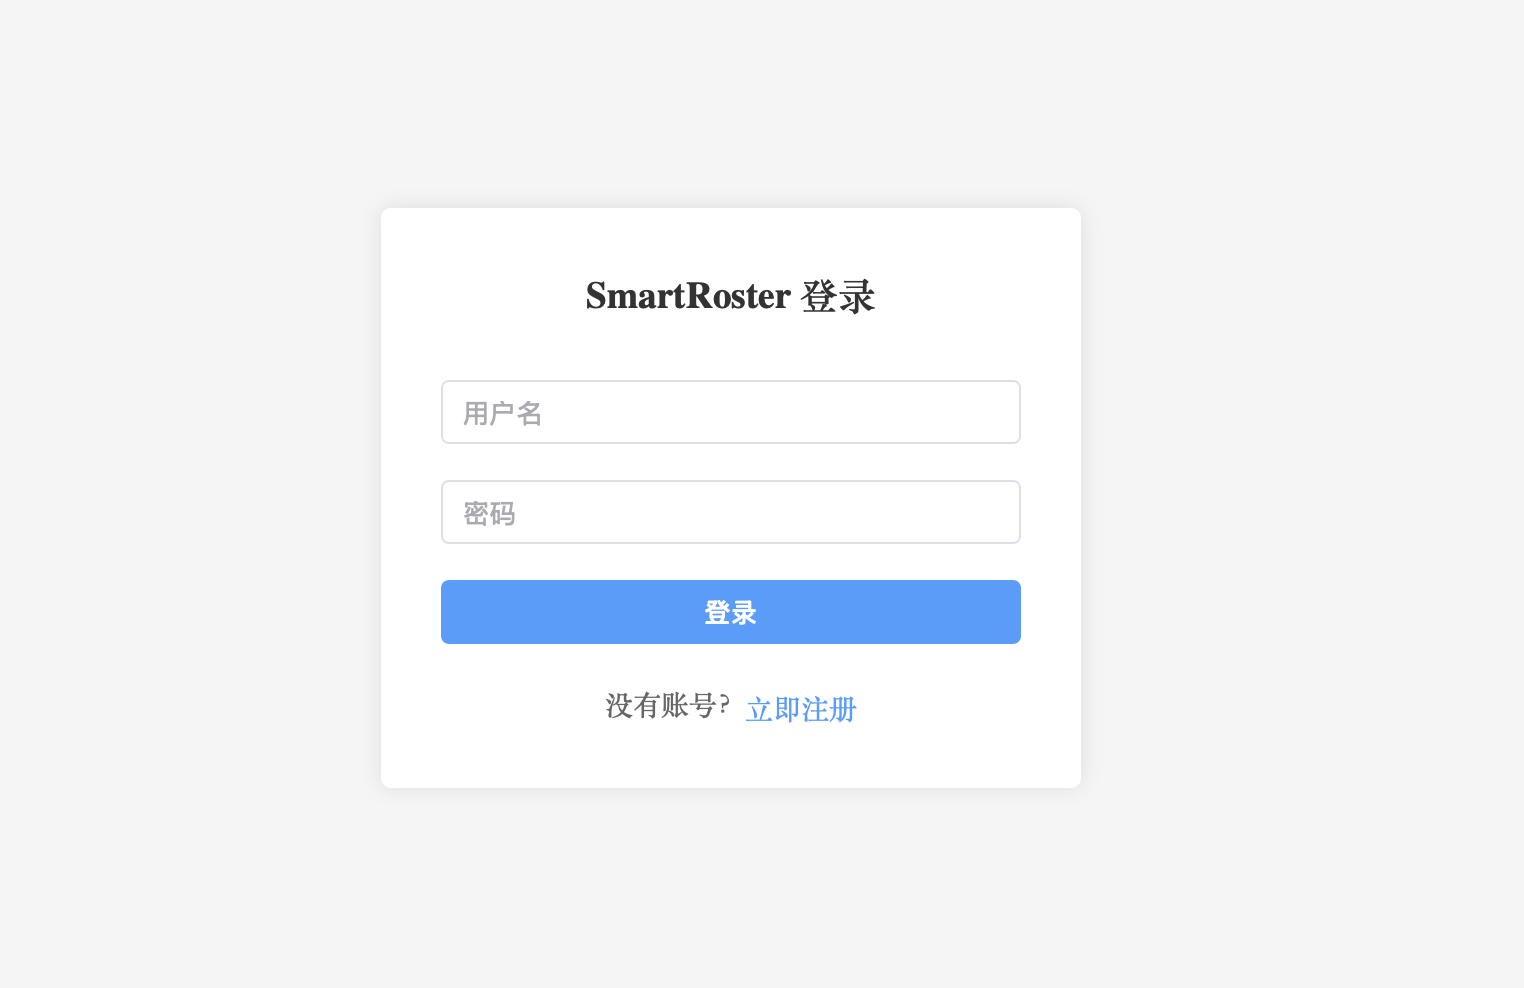
\includegraphics[width=0.8\linewidth]{./source/登录界面.png}
    \caption{登录界面}
    \label{fig:microservice-arch}
\end{figure}
\begin{figure}[H]
    \centering
    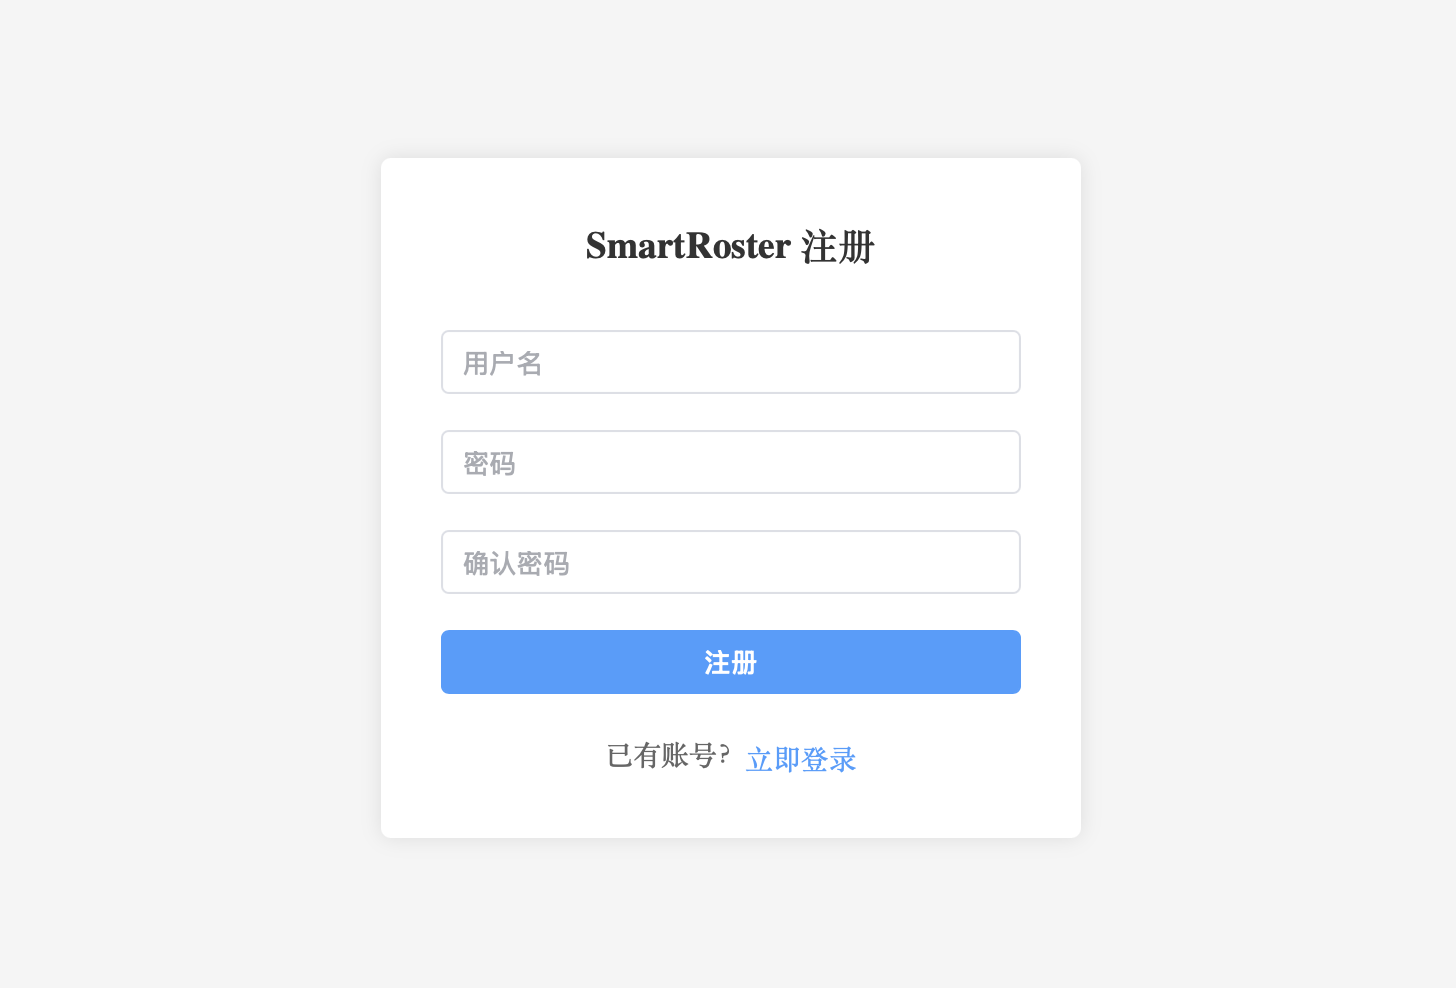
\includegraphics[width=0.8\linewidth]{./source/注册界面.png}
    \caption{注册界面}
    \label{fig:microservice-arch}
\end{figure}
\begin{figure}[H]
    \centering
    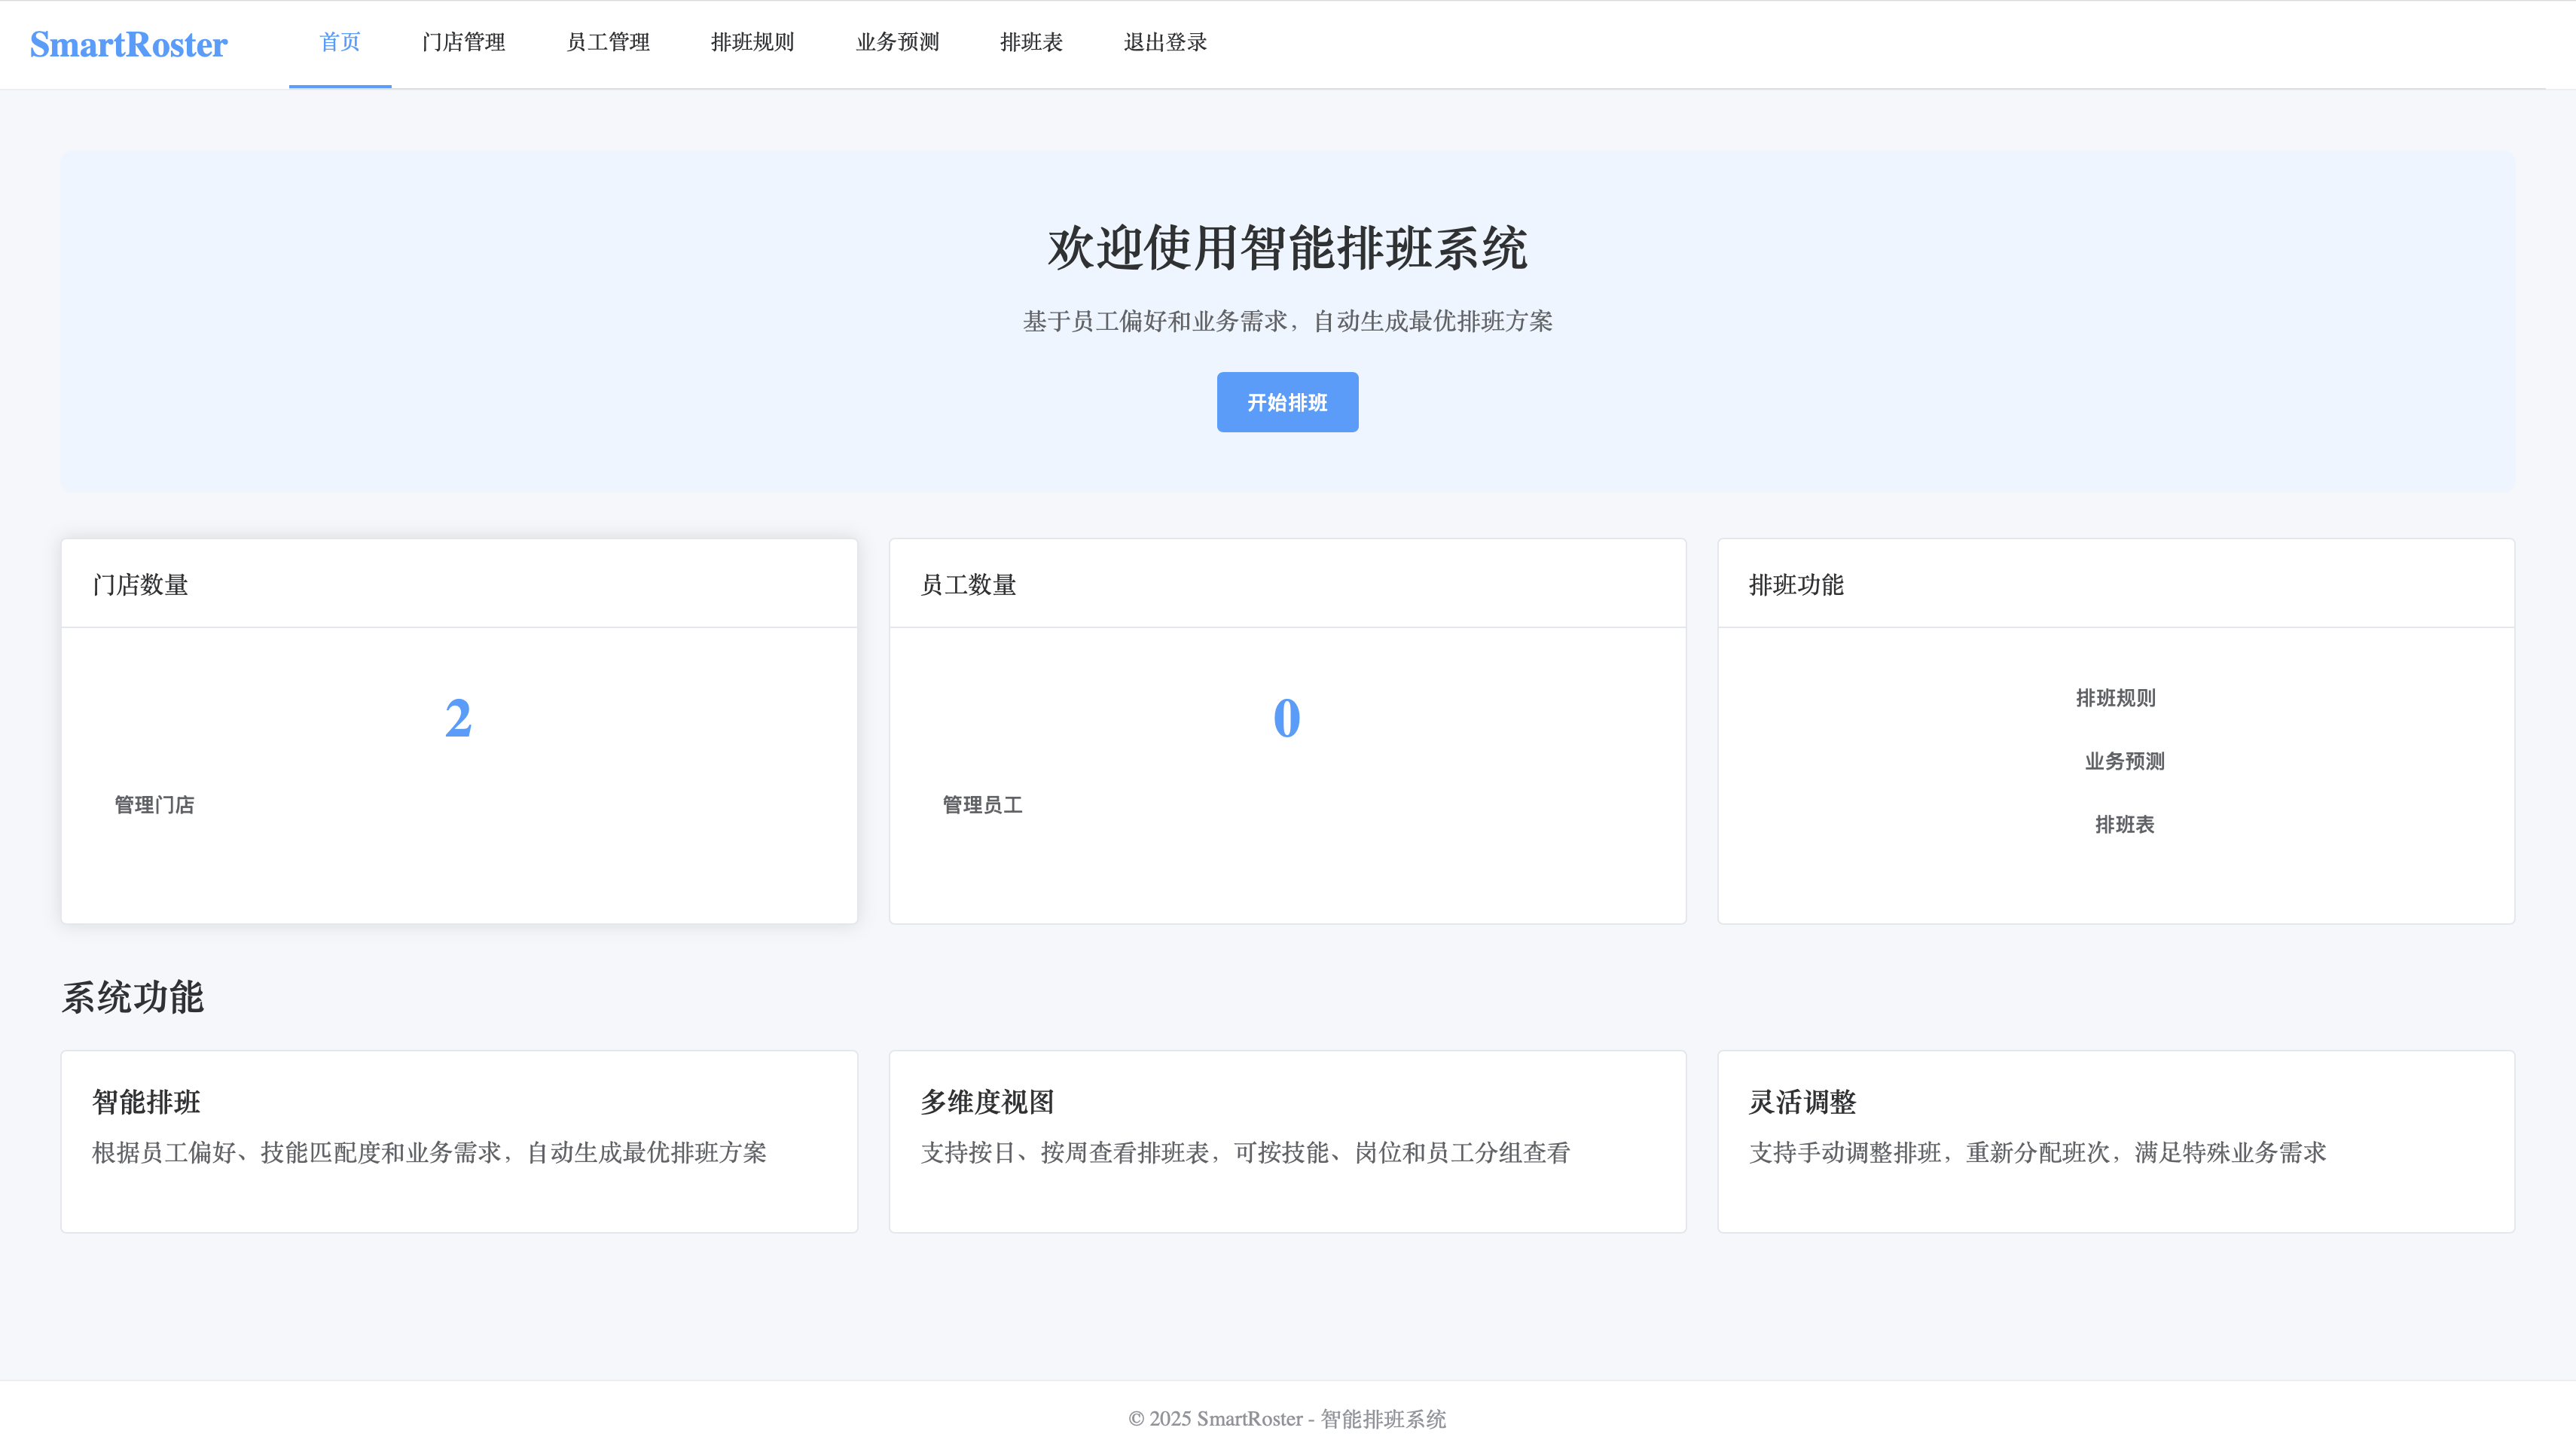
\includegraphics[width=0.8\linewidth]{./source/主页.png}
    \caption{主页}
    \label{fig:microservice-arch}
\end{figure}
\begin{figure}[H]
    \centering
    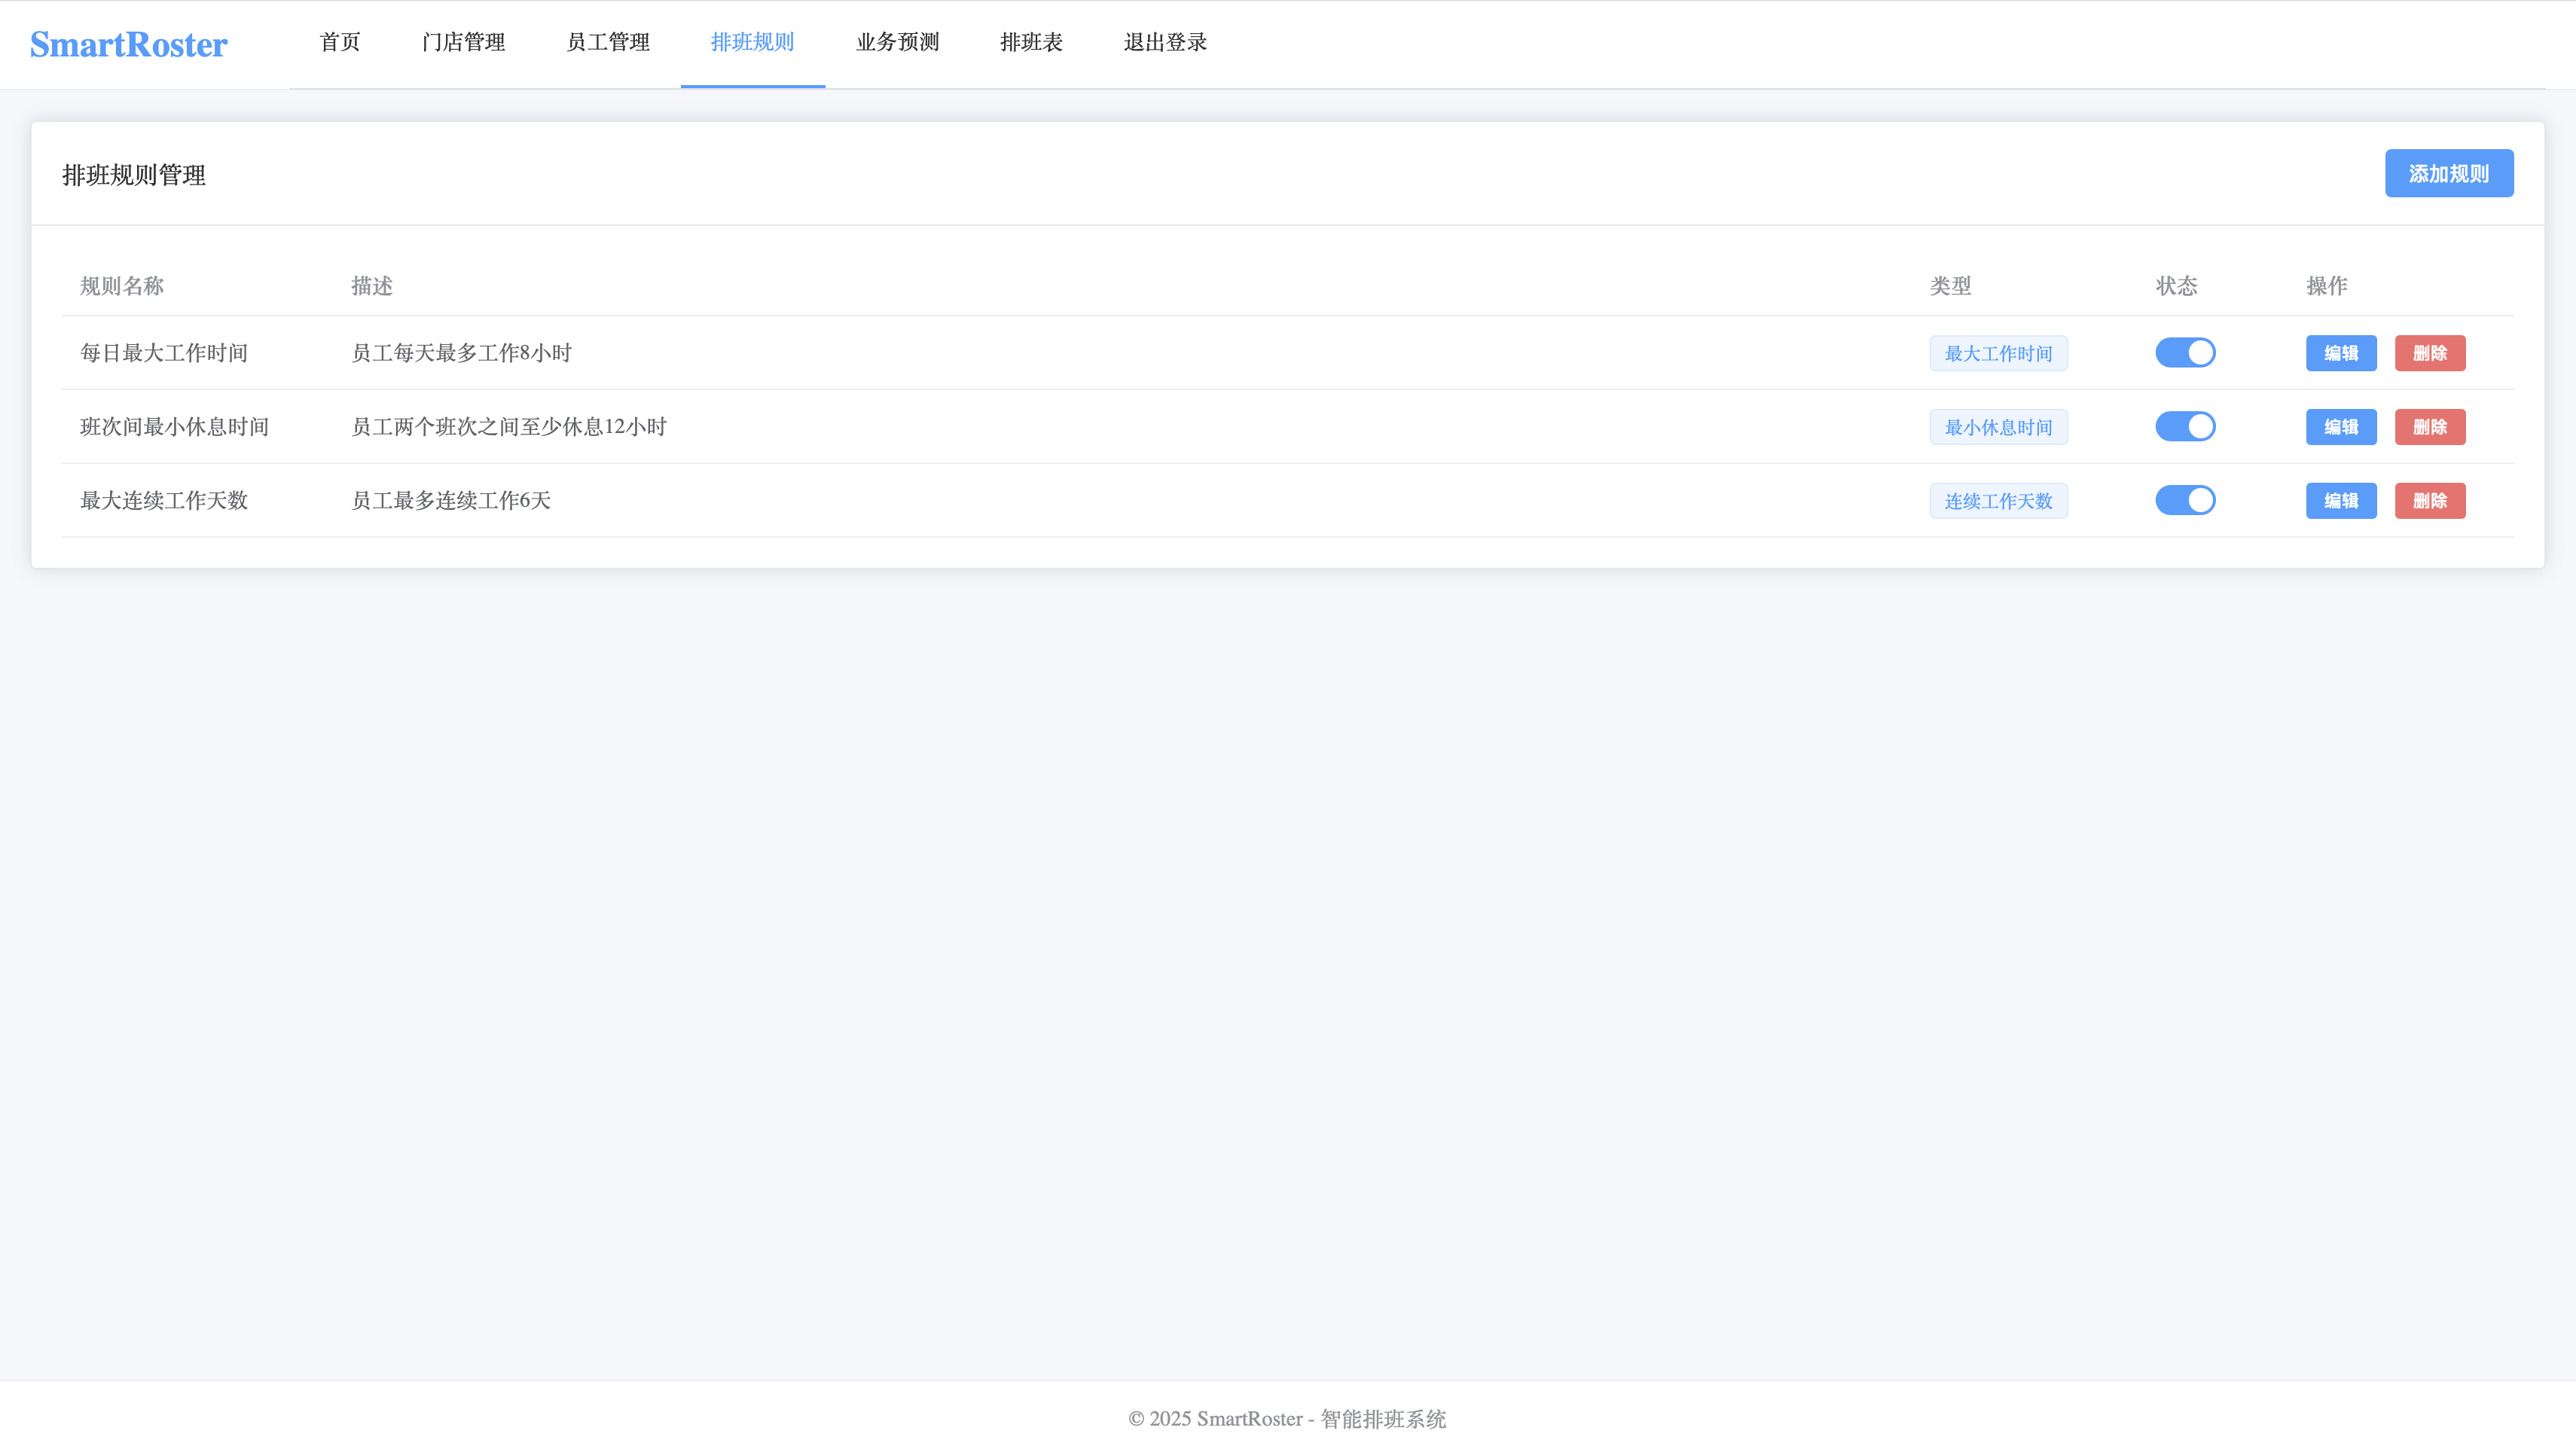
\includegraphics[width=0.8\linewidth]{./source/排班规则管理.png}
    \caption{排班规则管理}
    \label{fig:microservice-arch}
\end{figure}


\section{结论}


% 致谢
\section*{致谢}
\addcontentsline{toc}{section}{致谢}

% 参考文献
\addcontentsline{toc}{section}{参考文献}
\bibliographystyle{gbt7714-numerical} % 中文参考文献样式
\bibliography{references} % 指定参考文献数据库文件

% % 附录
% \appendix
% \addcontentsline{toc}{section}{附录A:系统功能模块详细说明}
% % 这里添加附录内容

% \addcontentsline{toc}{section}{附录B:核心算法伪代码}
% % 这里添加附录内容

\end{document}
